%%%%%%%%%%%%%%%%%%%%%%%%%%%%%%%%%%%
%%%Compile with XeLaTeX
%%%%%%%%%%%%%%%%%%%%%%%%%%%%%%%%%%%

\documentclass[11pt,twocolumn,openany,leqno]{e61-research-note}

\pagestyle{e61}

\usepackage{lipsum}

\addbibresource{references.bib}

\begin{document}

\emergencystretch=5pt
\baselineskip=15pt
\sloppy

\title{Example research note title}
% The title figure is controlled by "title_figure.pdf" in /figures/

\SubTitle{e61 Research Note No. XX}

\author{Author 1 and Author 2}

\maketitle

\chapter*{Summary}

\begin{abstract}

\lipsum[1-2]

\end{abstract}

\chapter{\lipsum[][1]}

\lipsum[1] \parencite{Adams22}.

\lipsum[2] (Figure \ref{fig:j2j-agg}). 

\newpage

\begin{Boxx}[label=b1]{Literature review}
\begin{small}
\setlength{\parindent}{15pt}
\lipsum[3-4]
\end{small}
\end{Boxx}

\begin{figure}[htb]
\caption{Job-to-job Transition Rates}\label{fig:j2j-agg}
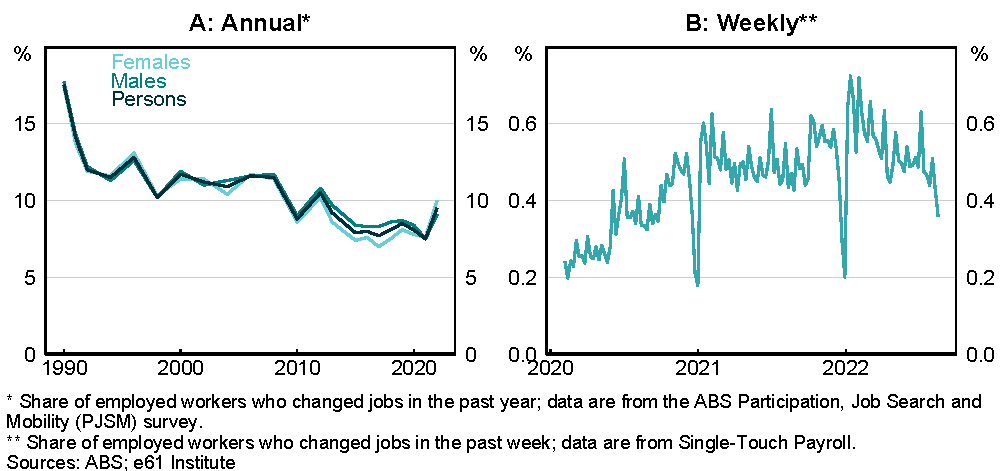
\includegraphics[width=0.95\columnwidth]{sample fig 1.pdf}
\end{figure}

\chapter{\lipsum[][2]}

\lipsum[][1]
\begin{enumerate}
  \item \lipsum[][4]
  \item \lipsum[][5]
\end{enumerate}

\lipsum[1] (see Appendix \ref{app:reg} for further details).

\lipsum[2]\footnote{\lipsum[][1-4]}

\lipsum[3]

\begin{figure}[htb]
\caption{Wage Outcomes From Job Transitions}\label{fig:stp-wages}
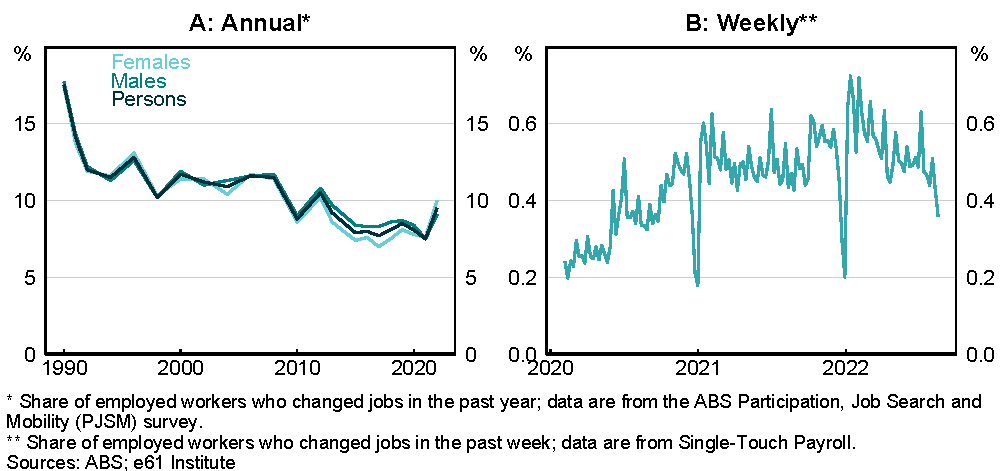
\includegraphics[width=\columnwidth]{sample fig 1.pdf}
\end{figure}

\newpage

\begin{Boxx}[label=box-pay]{Moves to higher paying firms and pay-setting mechanisms}
%\setlength{\parindent}{15pt}
\setlength{\parskip}{\baselineskip}

\lipsum[8-12]

\begin{minipage}{\textwidth}
  \captionof{figure}{Share of Transitions to Higher Paying Jobs}\label{fig:award-trans}
  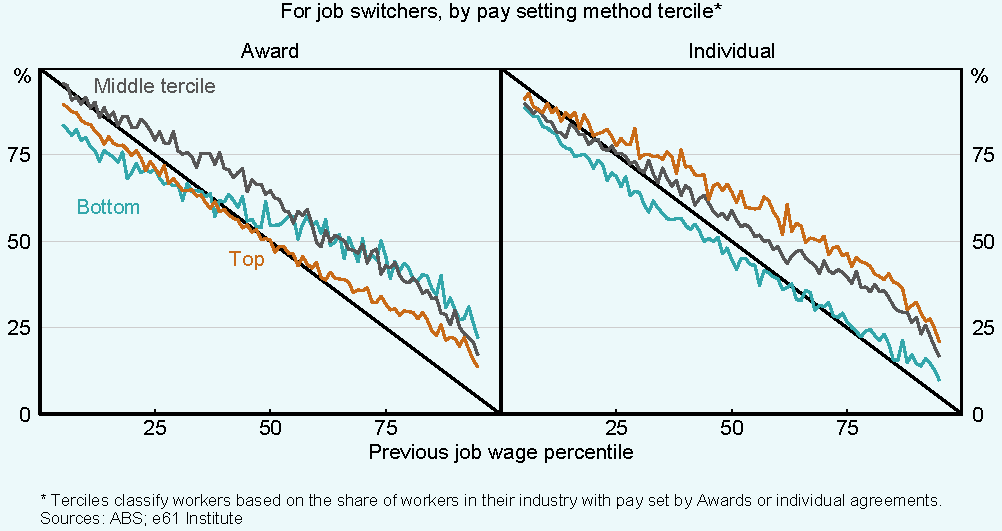
\includegraphics[width=\linewidth]{sample fig 2.pdf}
\end{minipage}

\end{Boxx}

\chapter{\lipsum[][10]}

\lipsum[1-6]

\printbibliography[title={References}]

\begin{appendix}

\chapter{Regression specifications and tables}
\label{app:reg}

This section provides additional detail on the econometric approach taken and associated outputs. There are two relationships we are interested in exploring:
\begin{itemize}
    \item Wage equation: the association between a worker’s decision to switch jobs and the change in their wage between their old and new job.
    \item Productivity equation: the association between a worker’s decision to switch jobs and the difference in productivity at their old and new firm.

\end{itemize}

In both these regressions, the outcome is a relative difference compared to a worker who does not make a job switch.

The specifications for the regressions are as follows:
\begin{align}
    \Delta wage_{it} &= \beta\left(switch\right)_{it}+\gamma_{it}+\lambda_{rt}+\epsilon_{it} \\
    \Delta prod_{it} &= \beta\left(switch\right)_{it}+\gamma_{it}+\lambda_{rt}+\epsilon_{it}
\end{align}

Where:

\begin{itemize}
    \item For the $i$th worker and week $t$.
    \item $\left(switch\right)_{it}$ is an indicator variable that takes a value of 1 if the worker switches jobs in that time period and 0 otherwise.
    \item $\Delta p{\rm rod}_{it}=\ln{\left(\frac{prod_{it}}{prod_{it-1}}\right)}$ is the log-change in firm labour productivity between the previous and current job.
    \item $\Delta w{\rm age}_{it}=\ln{\left(\frac{wage_{it}}{wage_{it-1}}\right)}$ is the log-change in wages between the previous and current job.
    \item $\gamma_{it}$ represents industry-state-time fixed effects for the firm that the worker switches to, controlling for the state-specific industry trends. Industries are defined using 4-digit ANZSIC codes.
    \item $\lambda_{rt}$ are SA4 fixed effects controlling for geographical differences across the places of residence of workers.
\end{itemize}

Each regression is run with sub-samples of the data, the samples are all the combinations of:
\begin{itemize}
    \item Gender: Female, Male and Total
    \item Age: under 25, 25-34, 35-44, 45-54, over 55, and Total
\end{itemize}

For a total of 18 regressions for each left-hand-side variable.

{\renewcommand{\arraystretch}{1.1}
\tabcolsep=1.0\tabcolsep
\begin{table*}[p]
  \centering
  \caption{STP wages gender/age pair regressions}
    \begin{tabular}{lcccccccccc}
    \toprule
          & (1)   & (2)   & (3)   & (4)   & (5)   & (6)   & (7)   & (8)   & (9)   & (10) \\
\cmidrule{2-11}          & \multicolumn{10}{c}{Female} \\
\cmidrule(lr){2-3} \cmidrule(lr){4-5} \cmidrule(lr){6-7} \cmidrule(lr){8-9} \cmidrule(lr){10-11}          & \multicolumn{2}{c}{<25} & \multicolumn{2}{c}{25-34} & \multicolumn{2}{c}{35-44} & \multicolumn{2}{c}{45-54} & \multicolumn{2}{c}{55+} \\
    \midrule
    Switched jobs & 0.2504*** & 0.2411*** & 0.0909*** & 0.0873*** & 0.0379*** & 0.036*** & -0.0194 & -0.0202 & -0.0839 & -0.0856 \\
          & (0.005) & (0.005) & (0.0049) & (0.0049) & (0.0063) & (0.0063) & (0.007) & (0.007) & (0.0088) & (0.0088) \\
    \midrule
    Industry x State x Time FE & No    & Yes   & No    & Yes   & No    & Yes   & No    & Yes   & No    & Yes \\
    SA4 region FE & No    & Yes   & No    & Yes   & No    & Yes   & No    & Yes   & No    & Yes \\
    \midrule
    N     & 4,598,364 & 4,598,364 & 8,349,917 & 8,349,917 & 7,678,780 & 7,678,780 & 7,097,933 & 7,097,933 & 6,930,408 & 6,930,408 \\
    R2    & 0.002 & 0.044 & 0.000 & 0.019 & 0.000 & 0.020 & 0.000 & 0.024 & 0.000 & 0.026 \\
    Within R2 &       & 0.002 &       & 0.000 &       & 0.000 &       & 0.000 &       & 0.000 \\
    \midrule
          & (11)  & (12)  & (13)  & (14)  & (15)  & (16)  & (17)  & (18)  & (19)  & (20) \\
\cmidrule{2-11}          & \multicolumn{10}{c}{Male} \\
\cmidrule(lr){2-3} \cmidrule(lr){4-5} \cmidrule(lr){6-7} \cmidrule(lr){8-9} \cmidrule(lr){10-11}          & \multicolumn{2}{c}{<25} & \multicolumn{2}{c}{25-34} & \multicolumn{2}{c}{35-44} & \multicolumn{2}{c}{45-54} & \multicolumn{2}{c}{55+} \\
    \midrule
    Switched jobs & 0.2489*** & 0.2431*** & 0.0885*** & 0.0844*** & 0.0053 & 0.0019 & -0.0296 & -0.0319 & -0.0607 & -0.0626 \\
          & (0.0051) & (0.005) & (0.004) & (0.004) & (0.0049) & (0.0048) & (0.0056) & (0.0056) & (0.0068) & (0.0067) \\
    \midrule
    Industry x State x Time FE & No    & Yes   & No    & Yes   & No    & Yes   & No    & Yes   & No    & Yes \\
    SA4 region FE & No    & Yes   & No    & Yes   & No    & Yes   & No    & Yes   & No    & Yes \\
    \midrule
    N     & 4,461,925 & 4,461,925 & 9,014,800 & 9,014,800 & 8,621,240 & 8,621,240 & 7,269,637 & 7,269,637 & 7,367,180 & 7,367,180 \\
    R2    & 0.002 & 0.042 & 0.000 & 0.023 & 0.000 & 0.025 & 0.000 & 0.026 & 0.000 & 0.022 \\
    Within R2 &       & 0.002 &       & 0.000 &       & 0.000 &       & 0.000 &       & 0.000 \\
    \bottomrule
    \end{tabular}%
  \label{tab:wages1}%
\end{table*}%
}

\chapter{Disclaimer}

\section*{Business Longitudinal Analysis Data Environment (BLADE)}
This paper uses unit record data held in the BLADE data environment which is hosted by the Australian Bureau of Statistics. The results are based, in part, on Australian Business Register (ABR) data supplied by the Registrar to the Australian Bureau of Statistics (ABS) under A New Tax System (Australian Business Number) Act 1999 and tax data supplied by the Australian Taxation Office (ATO) to the ABS under the Taxation Administration Act 1953. These require that such data are only used for the purpose of carrying out functions of the ABS. No individual information collected under the Census and Statistics Act 1905 is provided back to the Registrar or ATO for administrative or regulatory purposes. Any discussion of data limitations or weaknesses is in the context of using the data for statistical purposes, and is not related to the ability of the data to support the ABR or ATO's core operational requirements. Legislative requirements to ensure privacy and secrecy of this data have been followed. Only people authorised under the Australian Bureau of Statistics Act 1975 have been allowed to view data about any particular firm in conducting these analyses. In accordance with the Census and Statistics Act 1905, results have been confidentialised to ensure that they are not likely to enable identification of a particular person or organisation.

\end{appendix}

\end{document} 